\documentclass{article}
\usepackage{graphicx} % Required for inserting images
\usepackage[unicode]{hyperref}
\usepackage[onehalfspacing]{setspace}           % 1.5 distance between lines
\usepackage{palatino}                           % font
\usepackage{tabularx}
\usepackage{tabu}
\usepackage{longtable}[=v4.13]

\bibliographystyle{plain}

\title{TDT Project Documentation}
\author{Stanciu Alin, Pricop Laurentiu}
\date{Academic Year 2023-2024, Spring Semester}

\begin{document}
\pagenumbering{roman}

\maketitle
\tableofcontents

\newpage
\pagenumbering{arabic}

\section{Application Details. Investigated features}

The application we are testing is called Physical Mail Manager. The application is available for fiddling around with publicly \cite{PmailSite}, and its code is available on GitHub \cite{PmailGithub}. We will refer to the app as "PMail" from now on.

PMail intends to provide a means of keeping track of physical mail (alternatively known as snail mail) that Laurentiu personally was sending and receiving. It allows configuring destinations and can assign to each letter a unique trackable code.

PMail provides the following features:
\begin{enumerate}
    \item Authentication based on username and password, along with registration.
    \item Maintain a list of receivers, along with information required on the envelope (address, full name, postal code) and other optional user-defined information.
    \item Store a list of letters. Each letter is attached to a receivers (which keeps the same name even if they are actually a sender), can store metadata such as letter unique code, price, and other optional user-defined information.
\end{enumerate}

In particular, we tested the following aspects of PMail:
\begin{itemize}
    \item Authentication (login/logout with password);
    \item Adding receivers;
    \item Adding letters;
    \item Grouping of letters based on receiver and type (sent/received).
\end{itemize}

\section{AC. IOs}

We are employees at a software agency, specializing in web software, in particular business-to-business solutions customized for each customer. The company lead has a middle-school child which came up with the idea of an application to manage snail mail they were constantly sending to their friends. Having some leftover allocation in the company, and being in the middle of a transition from Angular to React company-wide, the company lead figured that this idea is worth investigating further as a learning project for his engineers.

However, rather surprisingly, a specific market demand was identified for the application after development was complete. It seems the company's business partners can apply the software as an internal solution to manage mail going in and out of their headquarters.

The company lead wants to capitulate on this newfound demand, but the application is currently in an unfit state. As such, our company decided to expand the development team on the so-called PMail project and bring in some new roles. In particular, we, Laurentiu and Alin, were hired as QA engineers, which now have the task of identifying an initial round of bugs and issues found with the product after its initial, internal, launch.

Being an in-house and a training project, bugs are expected and the company lead insists on listing as many of them as possible. Additionally, the user interface and experience was an after-thought during development of PMail, so the company lead also wants to identify specific elements and flows of the application that might be a bit harder to grasp for a person unfamiliar with it, in the form of user experience hiccups.

\section{Testing Mission}

The initiative's goal is judging the app's fitness for releasing as a product of our company, and creating an improved version that can level up from the status of "learning project" to that of "marketable product". As QA engineers, we can only help with the first part.

We need to perform an initial assessment of the application, drawing up test cases around usual user behavior and also potential edge situations, while also investigating common user experience anti-patterns.

\section{Testing Strategy}

The strategy is fairly straightforward, and is broken up in two parts.

\begin{enumerate}
    \item API Black-Box Testing

          We are going to write integration tests for two functionalities of the application, that call APIs and test for proper responses and error messages.

          We limit ourselves to the API initially since we consider it to be the backbone of any web application, thus being of significant importance testing-wise.

          These tests try to uncover an assortment of types of bugs that relate to, but are not limited to, the following aspects: database connection, syntactically invalid data, semantically invalid data, incorrect references.

    \item User Experience: Exploratory Testing

          We are going to fiddle with the application's frontend, manually and in an exploratory manner, to try to uncover as many design anti-patterns as we can.

          We're going to make a list of behaviors that we identify as potential issues and hand it over to the company lead, which will decide what, if any, corrective actions are going to be taken for each of them.
\end{enumerate}

\section{Selected Test Design Techniques}

\begin{tabularx}{\textwidth}{|X|X|X|X|X|}
    \hline
    Part    & Test Strategy     & Test Design Technique  & Dimension Covered & Students and Features              \\
    \hline
    Part I  & Process-compliant & Beta Testing           & Coverage          & Laurentiu Pricop (Authentication)  \\
    \hline
    Part I  & Reactive          & Boundary Testing       & Risk              & Alin Stanciu (Adding letters)      \\
    \hline
    Part II & Reactive          & User Interface Testing & Risk              & Laurentiu Pricop (Authentication)  \\
    \hline
    Part II & Reactive          & User Interface Testing & Coverage          & Alin Stanciu (Adding destinations) \\
    \hline
\end{tabularx}

\section{Test Design. Test implementation. Test execution. Test Report}

\subsection{Test design}

\begin{longtabu}{X[1] X[1]|X[1] X[2] X[2]}
    \hline
    \textbf{Student} & \textbf{Feature} & \textbf{Test Design Technique} & \textbf{Details} & \textbf{Input, Expected Output} \\
    &&&&\\
    \hline
    \endhead
    Laurentiu Pricop & Authenti\-cation & Beta Testing & Can a normal user tinkering with the app with no intention to break it, break it? &
    \par \textbf{In:} create account
    \par \textbf{ExpOut:} account created
    \par \textbf{In:} login with valid credentials
    \par \textbf{ExpOut:} logged in
    \par \textbf{In:} login with invalid credentials
    \par \textbf{ExpOut:} error
    \\
    \hline
    Alin Stanciu & Adding letters & Boundary Testing & Is there a limit on the size of the address? Can letters be added in numerical fields? Is Unicode supported? Are SQL injections possible? &
    \par \textbf{In:} empty address
    \par \textbf{ExpOut:} error
    \par \textbf{In:} address very long
    \par \textbf{ExpOut:} error
    \par \textbf{In:} unicode text
    \par \textbf{ExpOut:} properly displayed
    \par \textbf{In:} SQL-like text
    \par \textbf{ExpOut:} properly displayed
    \par \textbf{In:} HTML-like text
    \par \textbf{ExpOut:} properly displayed
    \\
    \hline
    Laurentiu Pricop & Authenti\-cation & User Interface Testing & Are buttons readable and clear? Are CTA texts easily understandable? Are buttons responsive? &
    No explicit test cases can be drawn out.\\
    \hline
    Alin Stanciu & Adding receivers & User Interface Testing & Are buttons readable and clear? Are CTA texts easily understandable? Are buttons responsive? &
    No explicit test cases can be drawn out.
    \\
    \hline
\end{longtabu}

\subsection{Test implementation. Test execution}

\subsection{Test reports}

After running our devised tests, our tools (Postman and Testiny) can generate a series of test run reports. Screenshots of these reports are presented in Figures \ref{FigReportPostmanAuth}, \ref{FigReportPostmanLetters}, \ref{FigReportTestinyAuth}, \ref{FigReportTestinyReceivers}.

Full testing reports for Testiny are available in the TDT Project repository, while the Postman collection with the written tests is available in the same place.

\begin{figure}[htbp]
    \centering
    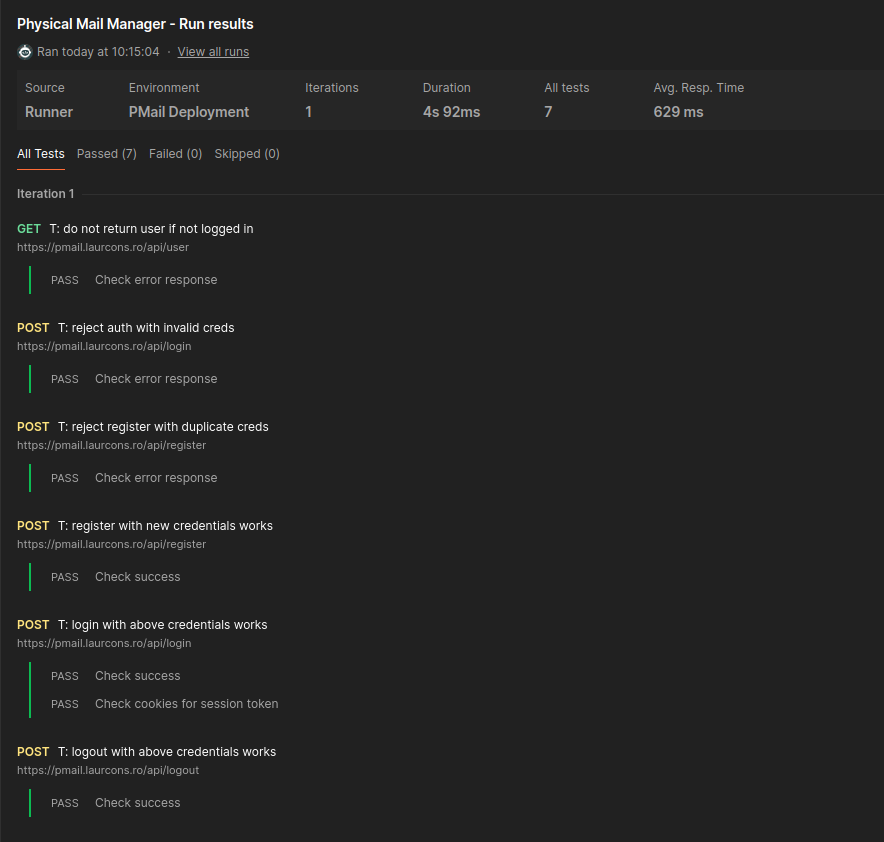
\includegraphics[width=0.7\textwidth]{./figures/postman-auth.png}
    \caption{Screenshot of run results for the Authentication feature, after running Beta Tests in Postman.}
    \label{FigReportPostmanAuth}
\end{figure}
\begin{figure}[htbp]
    \centering
    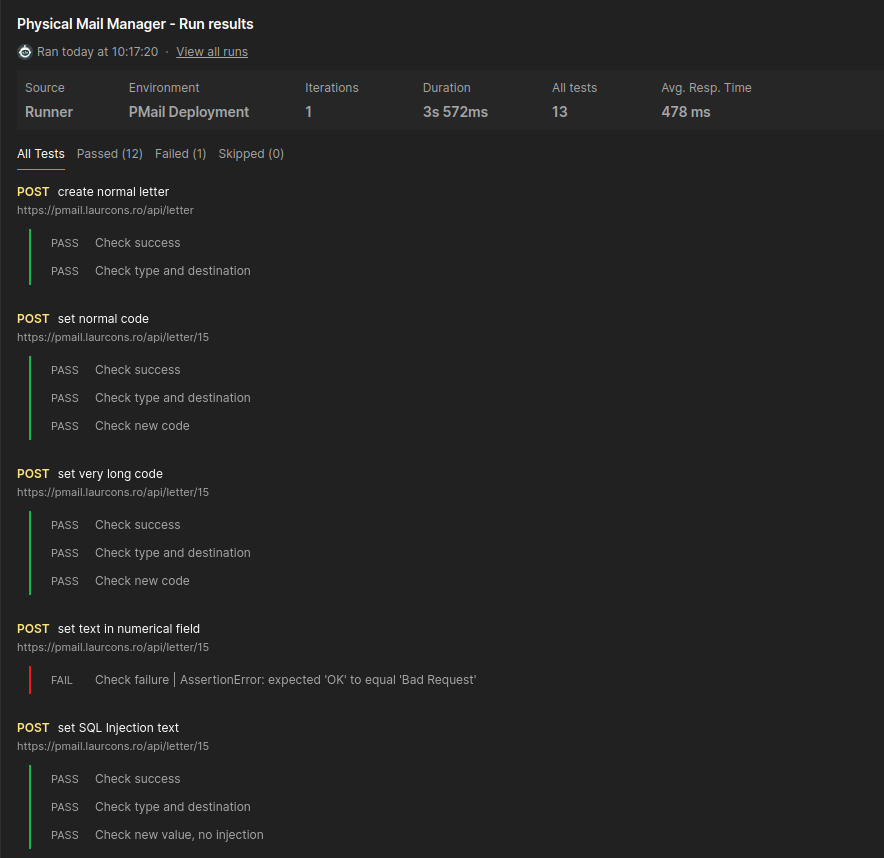
\includegraphics[width=0.7\textwidth]{./figures/postman-letters.png}
    \caption{Screenshot of run results for the Add Letter feature, featuring Boundary Testing with certain edge cases tested.}
    \label{FigReportPostmanLetters}
\end{figure}
\begin{figure}[htbp]
    \centering
    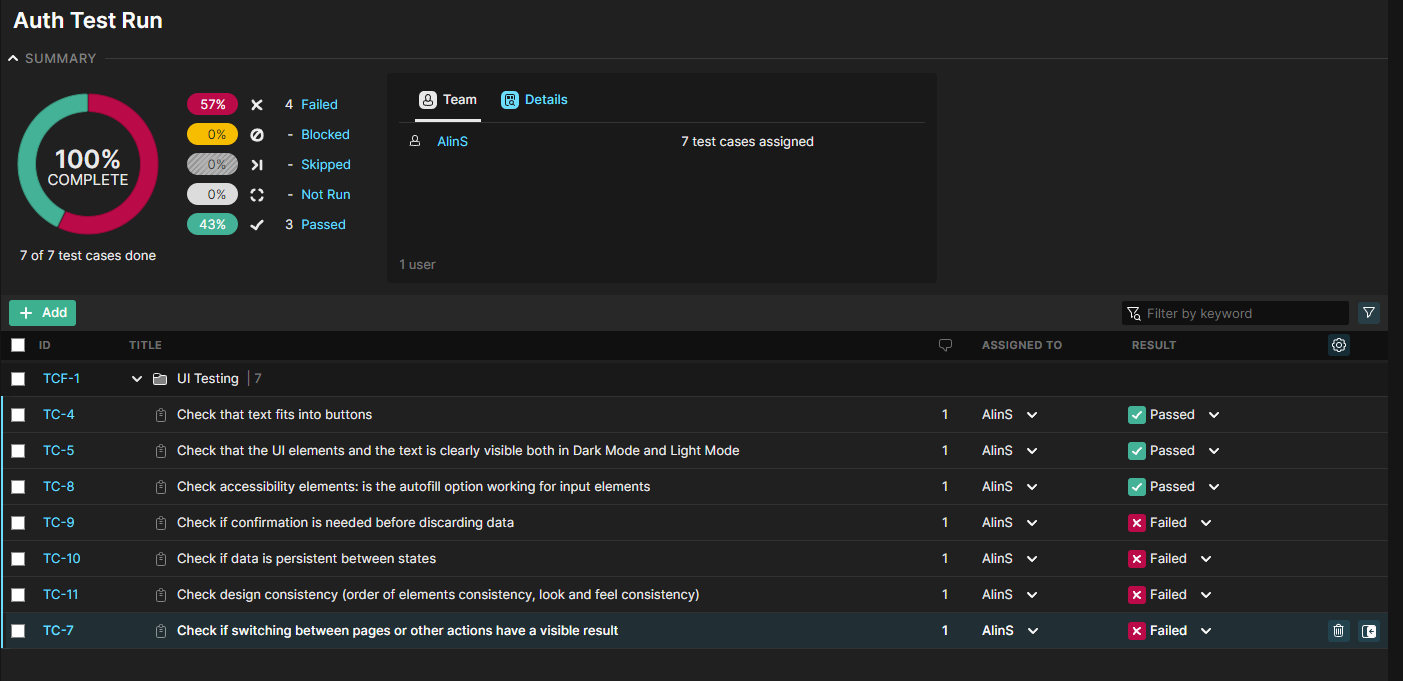
\includegraphics[width=0.9\textwidth]{./figures/testiny-auth.png}
    \caption{Screenshot of test run results for the Authentication feature, after manually running User Interface tests using Testiny.}
    \label{FigReportTestinyAuth}
\end{figure}
\begin{figure}[htbp]
    \centering
    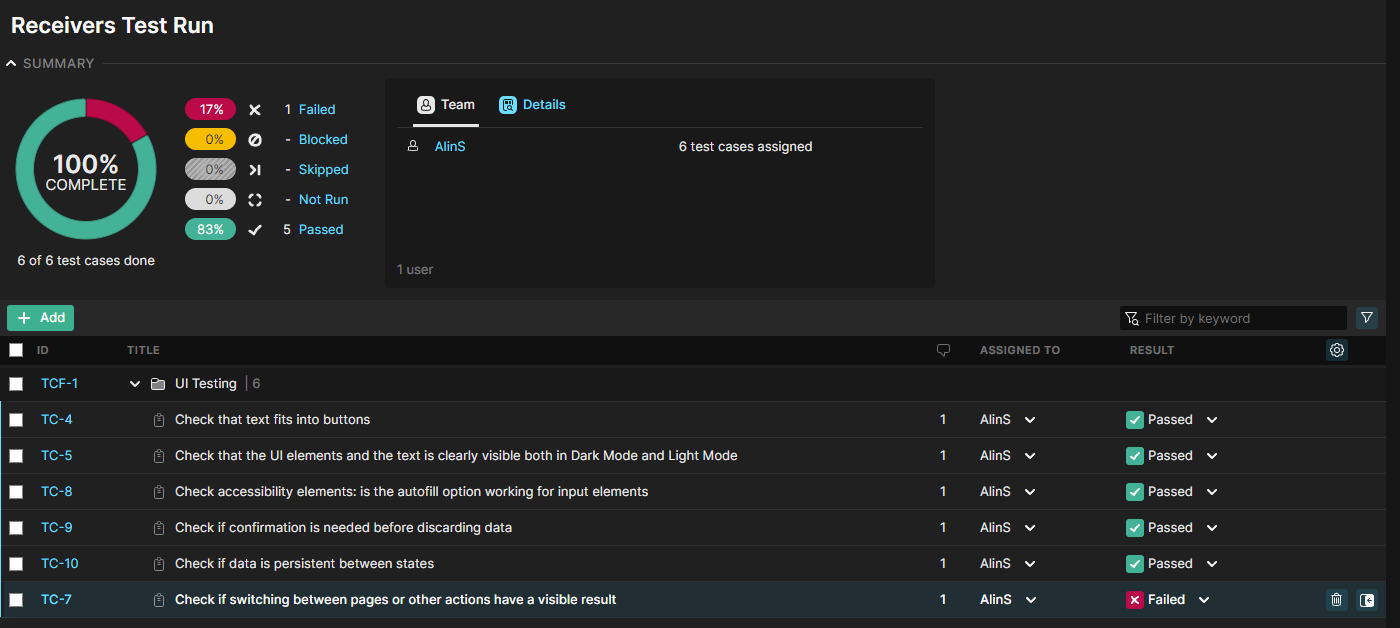
\includegraphics[width=0.9\textwidth]{./figures/testiny-receivers.png}
    \caption{Screenshot of test run results for the Add Receivers feature, after manually running User Interface tests using Testiny.}
    \label{FigReportTestinyReceivers}
\end{figure}

\section{Issue Reporting}

\section{Conclusions. Lessons Learned}

\newpage
\bibliography{references}

\end{document}
